\documentclass[11pt]{article}
\usepackage[utf8]{inputenc}
\usepackage{times}
\usepackage{geometry}
\usepackage{graphicx}
\usepackage{caption}
\usepackage{url}
\usepackage{hyperref}
\geometry{a4paper, margin=1in}

\title{Using Vision-Language Model for Top-k Precise Frame Identification in YouTube Videos}
\author{ NG Kin Pak\\
        \texttt{1155143402@link.cuhk.edu.hk}\and
        LI Yinxi\\
        \texttt{1155160255@link.cuhk.edu.hk}}
\begin{document}

\maketitle

GitHub Repository: \href{https://github.com/PeterNg2333/CSCI4140-CLIP-Frame-Identifier}{https://github.com/PeterNg2333/CSCI4140-CLIP-Frame-Identifier}

\section{Background and Problem Statement}
Efficiently locating and pinpointing specific moments within a sea of online video content, such as YouTube videos,
 remains a significant challenge in today's digital landscape. Traditional search methods, typically dependent on
  human-generated metadata or computational analysis based on visual and audio features, are constrained by their
   static nature and the labor-intensive processes involved. The innovative use of Vision-Language Models (VLMs), 
   like the Contrastive Language-Image Pre-training (CLIP) model, promises a transformative shift in enhancing video 
   searchability and accessibility. By harnessing the capabilities of VLMs, our system aims not just to find but to 
   precisely identify the top-k frames within videos that correspond to textual queries, facilitating efficient 
   navigation and rich user interaction with video content.


\section{Goals}
The primary goals of this project are:

\begin{enumerate}
    \item To implement a vision-language model (VLM) based system that significantly accelerates the
     process of identifying and retrieving specific video frames using textual queries, while maintaining 
     high accuracy and reliability.
    
    \item To innovate upon the existing capabilities of the CLIP model by exploring and incorporating 
    advanced techniques that enhance system performance, particularly in the context of speed and computational 
    efficiency.

    \item To design and develop a novel top-k classification approach, which may range from employing machine 
    learning clustering techniques for optimal case scenarios to designing alternative algorithms to ensure 
    diversity and coverage in result sets.
    
    \item To create an intuitive user interface and the system should be easy to use and guide users effectively 
    through the search process. The results page should be simple to navigate to the desired video frame.
    
    \item To contribute to the field of machine learning and computer vision by documenting the challenges 
    faced, methodologies used, and the impact of various optimization techniques on system performance.

\end{enumerate}



\section{Novelty}
The novelty of this project lies in its unique approach to video searching and frame identification. 
Unlike traditional methods that rely on predefined metadata or manual identification, our system leverages 
the power of Vision-Language Models to match video frames with textual descriptions in a real-time manner.
 Also, we will focus on enhancing the user experience of Vision-Language Models for precise frame identification 
 in videos content. 

 \section{Technical Challenges}

 The primary technical challenge in this project lies in enhancing the user experience — specifically in terms of speed, reliability, and diversification — of the Vision-Language Model (VLM) beyond the existing benchmarks set by the state-of-the-art (SOTA) models. While SOTA models such as CLIP already demonstrate robust performance, our goal is to push the boundaries further by exploring advanced optimization strategies. To this end, we plan to investigate various machine learning system enhancements such as:
 
 \begin{itemize}
     \item Intelligent Sampling: Developing algorithms for selective sampling of video frames that reduce the computational load without compromising the accuracy of the model.
     \item Repetition Reduction: Implementing mechanisms to recognize and avoid processing of repetitive content within videos, thereby increasing efficiency.
     \item State-of-the-Art (SOTA) Techniques: Testing and integrating the latest advancements in machine learning and computer vision to refine the model's performance, including real-time learning and adaptation to new video content types.
     \item Video Size Adaptability: Designing a robust system that can efficiently process and analyze videos of various sizes, especially those that exceed the typical processing capacity of current models. This involves creating strategies for the system to interact with users to specify a time range in case of oversized videos, ensuring continuous system operation without sacrificing user experience.
 \end{itemize}
 
 We recognize the complexity of these challenges, especially when considering the necessity to maintain a balance between computational efficiency and the accuracy of the model. It is crucial to achieve this balance to optimize the user experience. We will also address the challenges posed by large video files, ensuring that the system remains efficient and user-centric. This will include mechanisms to allow users to interact with the system to define processing parameters that align with the capabilities of the infrastructure while meeting their search needs. 

\section{Technical Impact}
The successful implementation of this project is expected to have a significant impact on the field of video content management and retrieval. By showcasing the effectiveness of VLMs in real-world applications, we aim to:

\begin{itemize}
    \item Illustrate the Versatility of VLMs: Demonstrate the wide array of practical applications for VLMs, encouraging developers to adopt and adapt these models for innovative uses.
    \item Propel Software Development: Provide a blueprint for integrating VLMs into software solutions, influencing future tools and platforms to leverage the full potential of vision and language understanding.
    \item Stimulate Research and Development: Inspire further research into optimization techniques for VLMs, potentially leading to breakthroughs that could benefit various domains such as online education, digital libraries, and content creation.
\end{itemize}

Through this project, we aim to not only advance the state of technology in video frame retrieval but also to provide a valuable reference for future research and commercial ventures in the domain of artificial intelligence and multimedia content processing.

\section{Social Impact}
By improving the searchability of video content, this technology can impact how information is consumed and shared with societies. There are several possible changes.  

\begin{itemize}
    \item Increased efficiency and accuracy in accessing video-based information. 
    \item Enhanced work productivity in research or jobs related to video. 
    \item Enhanced work productivity in research or jobs related to video. 
    \item Crime investigation  
\end{itemize}

\section{Methodology}
Our methodology will involve the use of several algorithms and libraries to achieve our objective: 

\begin{enumerate}
    \item Video Collection and Pre-processing: We will collect video from YouTuBe link (or users’ uploaded video) 
    and pre-process the video to extract frames which will involve using existing video processing libraries and tools to extract frames. (e.g. Decord, OpenCV, pytube, etc.) If the video is too large, the system will ask the user to specify a time range to process.
    
    \item Encoding Video: We will use the CLIP model to encode the video frames and the textual queries into a common embedding space. This will involve using the HuggingFace library to load the CLIP model and encode the video frames and textual queries. 
    
    \item Comparing Embedded Video Frames and Textual Queries: We will compare the embedded video frames and textual queries by Faiss which is a library for efficient similarity search and clustering of dense vectors. 
    
    \item Top-k Frame Identification: We will design and implement a novel top-k classification approach to identify the top-k frames that correspond to the textual queries. This will involve using machine learning clustering techniques or designing alternative algorithms to ensure diversity and coverage in result sets.
    
    \item System Implementation: we will apply Flask from Python for the lightweight backend framework and React for the interactive frontend. 


\end{enumerate}

\section{Evaluation Plan}

Our evaluation plan is designed to rigorously test the effectiveness and efficiency of the proposed system. 
It consists of several components that together will provide a comprehensive assessment of the project outcomes:

\begin{enumerate}
    \item Video Collection and Pre-processing: We will check the Youtube link and check the format of the returned video file to see if the system retrieved the correct video.
    
    \item Latency Measurement: We will measure the response time from when a query is submitted to when the results are displayed to the user. Our objective is to ensure that the system achieves a response as fast as it can for a seamless user experience.
    
    \item Diversity and Coverage Testing: We will test whether the user gets the desired number of top-k results and whether the variance of these results is as expected.
    
    \item User-Specified Time Range Functionality: To provide a tailored user experience, we will implement a feature allowing users to specify a time range for the video analysis. 
    This feature will be particularly useful for processing videos beyond the identified maximum size threshold. 
    The evaluation will test the system's capability to accurately process queries within these user-defined time ranges, ensuring that performance is not compromised when users interact with this functionality.
    
    \item Python server using Flask: We will develop a Python server using Flask to handle user queries and interact with the model. 
    
    \item User interface as web application: Our web application will emulate the matured and user-friendly interface of well-known platforms like YouTube. The search results will be displayed as thumbnails for each matching frame or video clip, with timestamps and relevance scores. Users will be able to click on a thumbnail to view the corresponding frame or clip, providing a user-centric and engaging interface. (For each query, the model could return continuous video clips that match the description.
    
    \begin{figure}[h]
        \centering
        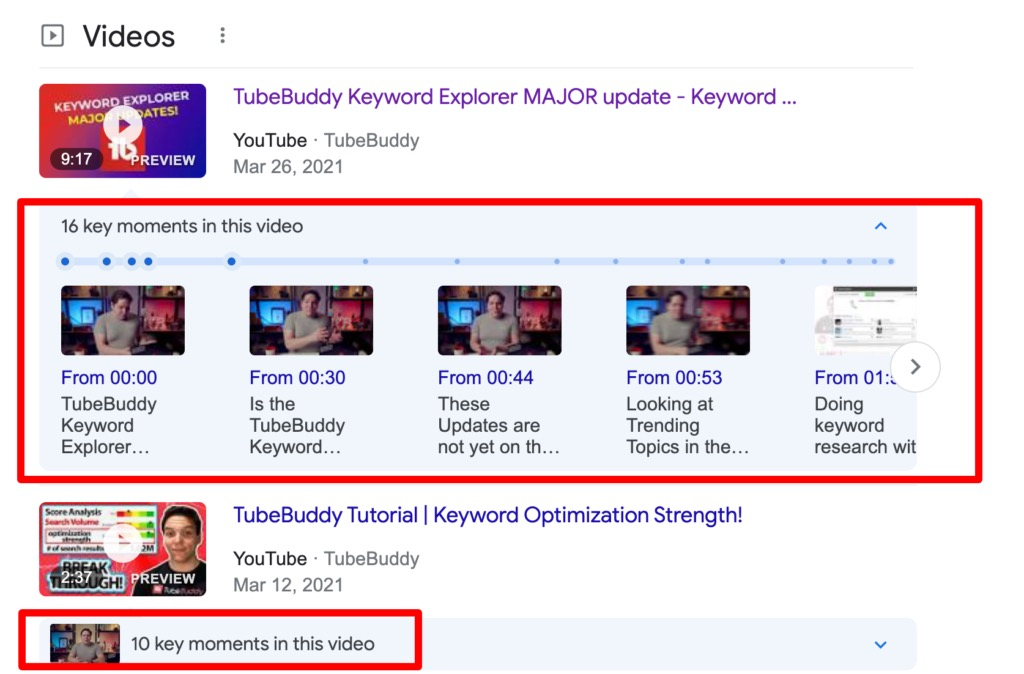
\includegraphics[width=\textwidth]{1.jpg}
        \caption{Demo search results, retrieved from \url{https://www.tubebuddy.com}}
        \end{figure}
    
\end{enumerate}
Each of these components will contribute to a holistic understanding of the system's performance and user experience. The findings from these evaluations will guide the iterative improvement of the system throughout the development process.

\section{Source}
\begin{itemize}
    \item OpenAI CLIP: \url{https://openai.com/clip/}
    \item Faiss: \url{https://github.com/facebookresearch/faiss}
    \item HuggingFace: \url{https://huggingface.co/}
    \item Decord: \url{https://github.com/dmlc/decord}
    \item OpenCV: \url{https://opencv.org/}
    \item pytube: \url{https://github.com/pytube/pytube}
    \item Flask: \url{https://flask.palletsprojects.com/en/2.0.x/}
    \item React: \url{https://reactjs.org/}
\end{itemize}

\end{document}

